%%%%%%%%%%%%%%%%%%%%%%%%%%%%%%%%%%%%%%%%%%%%%%%%%%%%%%%%%%%%%%%%%%%%%%%%%%%%%%%%
%% File   : skoranne_complex_hw7.tex
%% Author : Sandeep Koranne
%% Purpose: HW7 for complex analysis, good luck
%%%%%%%%%%%%%%%%%%%%%%%%%%%%%%%%%%%%%%%%%%%%%%%%%%%%%%%%%%%%%%%%%%%%%%%%%%%%%%%%
\documentclass{article}[12pt]
\usepackage{amssymb}
\usepackage{amsmath}
\usepackage{amsfonts}
\usepackage{amsthm}
\usepackage{a4wide}
\usepackage{polynom}
\usepackage{tikz}

%\usepackage[margin=1.5in]{geometry}
\newtheorem{lem}{Lemma}
\def\RR{\mathbb R}
\def\QQ{\mathbb Q}
\def\DD{\mathbb D}
\def\Aut{\mathrm{Aut}}
\def\Inn{\mathrm{Inn}}
\def\Out{\mathrm{Out}}
\def\CC{{\mathbb C}}
\def\NN{{\mathbb N}}
\def\ZZ{{\mathbb Z}}
\def\Fix{\mathrm{Fix}}
\def\Spec{\mathrm{Spec}}
\def\D{\mathrm{d}}
\def\nsub{{\trianglelefteq}}
\DeclareMathOperator{\sign}{sign}
\begin{document}
\title{Spring 2016 Complex Analysis HW7}
\author{Sandeep Koranne}
\date{May 20, 2016}
\maketitle


\section*{Problem 1}
Let $f$ be analytic in the extended complex plane except for
finitely many points $\{z_1,z_2,\ldots,z_k\}$ (which may include
the point at infinity) and suppose that $f$ has a pole at each of
the points $z_j$.
\subsection*{Problem 1(a)} Show that for each finite point $z_j$
there is an integer $m_j$ such that $(z-z_j)^{m_j}f(z)$ has a
removable singularity at $z=z_j$.
\begin{proof}
Since $f$ is given to be analytic everywhere (including the
point at infinity) except for its poles (which may include the
point at infinity), and $f$ has a pole (removable singularity)
at each of the points, we have two possibilities to consider.
Either $f$ does not have an essential singularity at the point
at infinity, in which case using Liouville's theorem, it is a
bounded on the domain $\CC\setminus \{z_j\}$ and is constant.
This can be inferred from Liouville's theorem and the maximum
modulus principle. 

If $f$ has an essential singularity at the point of infinity, then
also consider the function $g(z)=f(1/z)$, which has a singularity
at 0. If $f$ has a pole of order $m$ at infinity, then $z^mg(z)$
can be made analytic at $z=0$ (using Riemann Removable Singularity
Theorem). Now we can apply Cauchy's Integral Theorem for derivatives
and Cauchy's estimate to bound a sufficiently high derivative of $f$.
Alternatively, since 0 is now a pole of finite order for $g(z)$, it
directly implies that the Taylor expansion of $g(z)$ around 0, cannot
have arbitrary large negative powers. We can repeat this argument
for each $z_j$, and conclude that for each $z_j$, there will exist
a Taylor expansion for $g(z)=f(1/z)$ around $z_j$, where 
the Taylor expansion of $g$ cannot have arbitrary large negative
powers, thus there will exist some $m_j$ such that $(z-z_j)^{m_j}g(z)$
is analytic, and thus $(z-z_j)^{m_j}f(z)$ has a removable singularity
at $z_j$.
\end{proof}

\subsection*{Problem 1(a)}Show that $f$ is a rational function: that is,
there exist polynomials $p$ and $q$ such that $f=p/q$ on $\CC$ less
the set of poles.
\begin{proof}
This is proven in Simon for a a region $\Omega$ in Theorem 3.9.1~pp.~129
and also more generally in Section 9.5. We present essentially the
same argument below.
As given in the hypothesis $f$ has finitely many zeros and finitely many
poles, therefore we can consider the set of zeros of $f$ as
$\{a_1,a_2,\ldots,a_n\}$, while the set of poles is as given.
Consider another function $g(z)$ given as:
\[
g(z)= \frac{\prod_{i=1}^n (z-a_i)}{\prod_{j=1}^k (z-z_j)}
\]
Now $g(z)$ has the same zeros and poles as $f$, with the same 
multiplicities, therefore we can now consider $h(z)=\frac{f(z)}{g(z)}$
as a meromorphic function $h:\CC\to\CC$, which is defined
everywhere and in particular has no poles or zeros on $\CC^*$, where
$\CC^*$ is the extended complex plane. 
Then, by Liouville's theorem,
since $h(z)$ is a bounded entire function, it must be a constant,
thus $h(z)=c$, but this implies that $f=cg(z)$, and thus $f$ is
a rational function.
\end{proof}

\section*{Problem 2(a)} Evaluate the following sums for $a>0$
\[
\sum_{n=-\infty}^\infty (n^2+a^2)^{-2}
\]
\begin{proof}
We use the following result without proof (it is Theorem 5.7.13
of Simon~pp.~212).
\begin{lem}
Let $f$ be a rational function $f(z)=P(z)/Q(z)$, where
(i) $\mbox{deg}(Q) \ge 2+\mbox{deg}(P)$ and (ii) $P$ and $Q$
have no common zeros and $Q$ is non-vanishing at every $n\in\ZZ$,
then:
\[
\sum_{n=-\infty}^\infty f(n) = 
- \sum_{\mbox{zeros}\ z_k\ \mbox{of}\ Q} \mbox{Res}(fg;z_k)
\]
where $g(z)=\pi \cot(\pi z)$.
\end{lem}
The function $f(z)=\frac{1}{(n^2+a^2)^2}$, in the rational form $P(z)=1$
and $Q(z)=(z^2+a^2)^2$, meets the requirement of the Theorem above, and
we calculate the zeros $z_k$ of $Q$ as $\pm ia$. Therefore we have
\[
\sum_{n=-\infty}^\infty \frac{1}{(n^2+a^2)^2} + 
\mbox{Res}\left[\frac{\pi \cot(\pi z)}{(z^2+a^2)^2}; ia\right] +
\mbox{Res}\left[\frac{\pi \cot(\pi z)}{(z^2+a^2)^2}; -ia\right] = 0
\]
Since $f$ has a simple pole at $\pm ia$, using Theorem 5.7.13
we know $\mbox{Res}(fg;z_k)=g(z_k)\mbox{Res}(f;z_k)$.
We also know that $f=(z^2+a^2)^{-2}$ has residue 
$\frac{i}{4a^3}$ at $ia$, and $\frac{-i}{4a^3}$ at $-ia$.
Since $\cot$ is an odd function, we have the sum of the residues
is $-\frac{2i\pi\cot(\pi ia)}{4a^3}$, which we can simplify to
$-\frac{\pi\coth(\pi a)}{2a^3}$, therefore the first part of the infinite sum is
\[
\frac{\pi\coth(\pi a)}{2a^3}
\]
\end{proof}
We know that $\frac{d}{dz} \pi \cot(\pi z) = -\pi^2\csc(\pi z)^2$, therefore
the residue at $ia$ is $-\pi^2\csc(-i\pi a)^2$, while the residue at $-ia$
is $-\pi^2\csc(-i\pi a)^2$. Therefor the infinite sum is
\[
\sum_{n=-\infty}^\infty \frac{1}{(n^2+a^2)^2} = \frac{\pi\coth(\pi a)}{2a^3}+
\frac{\pi^2[\csc(i\pi a)^2]}{2a^3}
\]

\subsection*{Problem 2(b)} Evaluate the following sum for $a>0$
\[
\sum_{n=-\infty}^\infty (n^4+a^4)^{-1}
\]
\begin{proof}
Using similar technique as the previous problem, we first calculate the
zeros of $Q(z)$, where $f(z)=1/Q(z)$.
We can write the function as $f(z)=(z^4+a^4)^{-1}$, and factor the denominator
as $(z^4+a^4)=(z^2-ia^2)(z^2+ia^2)$.
The roots are $\omega:\omega^4+a^4=0$, let us denote them $\omega_1$
to $\omega_4$.
\[
(z^4+a^4) = (z-\omega_1)(z-\omega_2)(z-\omega_3)(z-\omega_4)
\]
and by comparing with the factoring, the roots are
\[
\omega_1 = \frac{1}{\sqrt{2}}(a-i), \omega_2 = \frac{-1}{\sqrt{2}}(a-i)
\]
\[
\omega_3 = \frac{1}{\sqrt{2}}(a+i), \omega_4 = \frac{-1}{\sqrt{2}}(a+i)
\]
The residue at the roots are given by the following:
\[
\mbox{Res}(f;\omega_1) = \lim_{z\to -\omega_1} (z+\omega_1)f(z)
\]
Using L'Hospital's rule
\[
\mbox{Res}(f;\omega_1) = \frac{1}{4\left[ \frac{1}{\sqrt{2}}(a+i)\right]^3} =
\frac{1}{2\sqrt{2}(1-i)a^3}
\]
By symmetry, the other residues are
\[
\mbox{Res}(f;\omega_2) = \frac{-1}{2\sqrt{2}(-1+i)a^3}
\]
\[
\mbox{Res}(f;\omega_3) = \frac{1}{2\sqrt{2}(1+i)a^3}
\]
\[
\mbox{Res}(f;\omega_4) = \frac{-1}{2\sqrt{2}(-1-i)a^3}
\]
Therefore the infinite sum is
\begin{eqnarray}
\sum_{n=-\infty}^\infty \frac{1}{(n^4+a^4)} & = & 
\pi\cot(\pi \frac{(a-i)}{\sqrt{2}}) \frac{1}{2\sqrt{2}(1-i)a^3}) -
\pi\cot(\pi \frac{(a-i)}{\sqrt{2}}) \frac{1}{2\sqrt{2}(-1+i)a^3}) -\nonumber \\
& & \pi\cot(\pi \frac{(a+i)}{\sqrt{2}}) \frac{1}{2\sqrt{2}(+1+i)a^3}) +
\pi\cot(\pi \frac{(a+i)}{\sqrt{2}}) \frac{1}{2\sqrt{2}(-1-i)a^3}) \nonumber
\end{eqnarray}
\end{proof}

\subsection*{Problem 2(c)} Evaluate the following sum for $a>0$
\[
\sum_{n=1}^\infty (n^4)^{-1}
\]
\begin{proof}
  Using the similar technique to problem (a) above we calculate the residue
  of $\pi\cot(\pi z)f(z)$, and therefore
  \[
  \sum_{n=\-infty}^\infty (n^4)^{-1} = \sum_{z_k} \mbox{Res} [\pi\cot(\pi z)f(z); z_k]
  \]
  Since the function is even, we can divide the sum of the residues by 2 to
  get our infinite sum. To get the residue we had to use the Laurent series
  around 0, as for other $n$, the integral $\int_C \frac{\pi \cot(\pi z)}{z^4}dz \to 0$
  as $N\to\infty$, using the Cauchy estimate for the integral.
  \[
  \lim_{N\to\infty} \frac{1}{2\pi i} \int_C \frac{\pi \cot(\pi z)}{z^4} dz = 0
  \]
  This gives us
  \[
  \sum_{n=-\infty}^\infty \mbox{Res}[\frac{\pi \cot(\pi z)}{z^4}; z=n] +
  \mbox{Res}[\frac{\pi\cot(\pi z)}{z^4}; z=0] = 0
  \]
  Therefore the
  only contribution to the infinite sum is from the residue around 0
  and we have $\sum_{n=1}^\infty \frac{1}{n^4} + \mbox{Res} [g(z);0] = 0$ (using
  the residue formula),
  and we have
  \[
  \frac{\pi \cot(\pi z)}{z^4} = \frac{\pi \cos(\pi z)\csc(\pi z)}{z^4} =
  \frac{\pi}{z^4}\left( 1-\frac{(\pi z)^2}{2!} +\frac{(\pi z)^4}{4!} + \cdots\right)
  \left(\frac{1}{\pi z} + \frac{\pi z}{6}+\cdots+\right)
    \]
    Comparing the series with terms of coefficients of $z^3$ in the numerator we get
    the sum is $\pi^4/45$, therefore the infinite sum is $\pi^4/90$.
  
\end{proof}

\section*{Problem 3: Simon p.~221, problem 20}
 This problem will provide an alternative
proof of the strong form of the Nyquist-Shannon sampling theorem.
Suppose $f(z)$ is an entire function obeying
\[
|f(z)| \le C \exp((\pi-\epsilon)|\mbox{Im}z|)
\]
Fix $z_0\in \CC\setminus \ZZ$. Let
\[
g(z)=\frac{f(z)}{(z-z_0)\sin(\pi z)}
\]
and let $R_k$ be the rectangle which is the boundary 
of $\{x+iy|\ |x|\le k+\frac{1}{2}, |y|\le k+\frac{1}{2}\}$, oriented
clockwise.
\begin{proof}
  Given $f(z)$ is an entire function such that $|f(z)|\le \exp(\pi r |\sin \theta|)$
  as $z$ approaches infinity, for $z=re^{i\theta}$, in other words,
  $|f(z)$ becomes infinite to a lower order than $e^{\pi r|\sin\theta|}$, in the
  words of Ogura, is equivalent to the hypothesis given above.
  Therefore we are considering functions which have no rapid oscillations and
  are bounded in strips parallel to the real axis.
  Now let $f$ have a pole of order 1 at $z_0$, so that near $z_0$ we can take
  $f$ to be of the form $f=f'(z)/(z-z_0)$, where $f'(z)$ is analytic in a
  neighborhood of $z_0$. If now we replace $f$ by $f'$ we have
  \[
  f^*(z) := f(z)-f'(z)\frac{\sin(\pi(z-a)/w)}{(z-z_0)\sin(\pi(z_0-a)/w)}
  \]
  where $\{a+rw\}$ are points in the sample space.
  Here $f^*(z)$ introduces no new singularities, and for all sufficiently
  large $|z|$ it remains bounded in strips parallel to the real axis.

  As given, we consider the rectangular contour considered clockwise,
  and $g$ is a function with simple poles at the integer values, $z=n$,
  for $n\in\ZZ$, then by the Cauchy residue theorem
  \[
  \lim_{k\to\infty} \int_{R_k} \frac{\pi f(z) \cos(\pi z)}{(z-z_0)} dz =
  \lim_{k\to\infty} \int_{R_k} \frac{\pi \cot(\pi z) f(z)}{z-z_0} dz =
  \lim_{k\to\infty} \int_{R_k} |g(z)| d|z| = 0
  \]
  
  We use without proof Lindel\"of's equation below:
  \[
  \sum_{k=-m}^m (-1)^k g(k) = \frac{1}{2\pi i}\int_C \frac{\pi}{\sin(\pi z)} g(z)dz
  - \sum_C \frac{\pi}{\sin(\pi z)}(g(z))
  \]
  
\end{proof}

\subsection*{Problem 3(a)}Prove that
\[
\lim_{k\to\infty} \int_{R_k}|g(z)|d|z|=0
\]
\begin{proof}

\end{proof}

\subsection*{Problem 3(b)}Prove that
\[
f(z_0)=\frac{\sin(\pi z)}{\pi} \lim_{k\to\infty} \sum_{n=-k}^k
\frac{(-1)^nf(n)}{z_0-n}
\]
which is (6.6.76) of Part 1.
\begin{proof}

\end{proof}

\section*{Problem 4}Let $f$ be a holomorphic map of the unit disk
to itself with $f(0)=0$. Let $m$ be the multiplicity of $z=0$ as
a zero of $f$. Prove that $|f(z)|\le |z|^m$.
\begin{proof}
In the following $\Omega$ is the closed unit disk.
We first state Schwarz's Lemma, as we will need it immediately.
If $f$ is analytic and satisfies $|f(z)|<1$ on $\Omega$
and $f(0)=0$, then $|f(z)|\le |z|$ for each $z\in\Omega$ with
equality iff $f$ has the form $f(z)=e^{i\theta}z$ for some $\theta\in\RR$.
Furthermore, $|f'(0)|\le 1$ with equality iff 
$f$ has the form $f(z)=e^{i\theta}z$ for some $\theta\in\RR$.

Since $f$ has a zero of order $m$ at the origin, we have
$f(0)=0=f'(0)=f''(0)=f^{(m-1)}(0)$, but $f^{(m)}(0)\ne 0$.
Then $f(z)=\sum_{k=m}^\infty a_kz^k$, where $a_k=f^{(k)}(0)/k!$, from
Taylor series coefficient formula.
But this implies that we can write $f(z)=z^mg(z)$ for all $z\in\Omega$
where $g(z)=\sum_{k=m}^\infty a_kz^{k-m}$.
This function $g(z)=f(z)/z^m$ has a removable singularity at the 
origin so that we can define $g(z)$ as
\[
g(z) = \left\{ \begin{array}{lc} f(z)/z^m\ & \mbox{for}\ z\in\Omega\setminus \{0\} \\
a_n & \mbox{for}\ z=0 \end{array}\right.
\]
Then $g$ is analytic on $\Omega\setminus\{0\}$ and also continuous
on $\Omega$. Using the Riemann Removable Singularity Theorem,
$g$ is analytic on $\Omega$. 
We also note that $g(z)\le 1$ for all $z\in\Omega$; this follows
from the maximum modulus principle because as given by the hypothesis
of the problem $f(z)\le 1$ on $\Omega$, therefore
\[
|g(z)| = \frac{|f(z)|}{|z|^m}|_{|z|=r} \le \frac{1}{r^m}
\]
by letting $r\to 1$, we get $g(z)\le 1$.
Now if $g(z)$ is bounded on $\Omega$, by the maximum modulus principle,
since $g$ attains its maximum at an interior point, $g$ must be a constant.
Therefore $g(z)=c$, where $|c|\le 1$. But this directly implies 
$\frac{f(z)}{z^m}\le 1$, which is equivalent to $f(z)\le z^m$, as
required.
\end{proof}

\section*{Problem 5}Evaluate the following integrals.
Hint: you can evaluate both (a) and (b) together
by integrating $z^{a-1}(1-z)^{-1}$ around a suitable contour
and taking the real and the imaginary parts.

\begin{figure}[htb]
\begin{center}
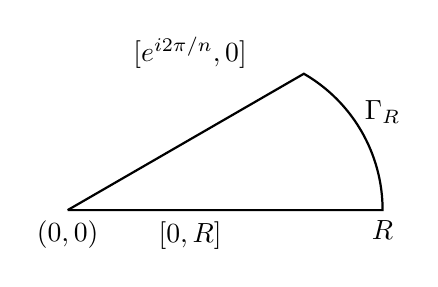
\begin{tikzpicture}
% Configurable parameters
\def\gap{0.2}
\def\bigradius{3}
\def\littleradius{0.5}

% Axes
%\draw [help lines,->] (-1.25*\bigradius, 0) -- (1.25*\bigradius,0);
%\draw [help lines,->] (0, -1.25*\bigradius) -- (0, 1.25*\bigradius);
%\path[draw,line width=0.8pt] (1,0) node[below] {$\varepsilon$} -- (2,0) node[below] {$r$} arc (0:180:2) -- (-1,0) arc (180:0:1);
\path[draw,line width=0.8pt] (0,0) node[below] {$(0,0)$} -- (4,0) 
node[below] {$R$} arc (0:60:2) -- (0,0);
\node at (1.555,-0.32) {$[0,R]$};
\node at (1.555,2) {$[e^{i2\pi/n},0]$};
\node at (4,1.25) {$\Gamma_R$};
\end{tikzpicture}
\caption{Contour for integration using residue theorem.}
\label{fig:residue-contour}
\end{center}
\end{figure}


We first prove the following Lemma, which will help us.
\begin{lem}
\[
\int_0^\infty \frac{x^{m-1}}{1+x^n} dx = \frac{\pi}{n \sin(m\pi/n)}
\]
\end{lem}
\begin{proof}
Consider $f(z)=\frac{z^{m-1}}{1+z^n}$, then $f$ has simple poles
at $a_k=e^{i(1+2k)\pi/n}$ for $k=0,1,\ldots,n-1$, and the residue
\[
\mbox{Res}[f(z); a_k] = \frac{z^{m-1}}{nz^{n-1}}|_{z=a_k} = \frac{-z^m}{n}|_{z=a_k}
= \frac{-a_k^m}{n}
\]
Next consider a contour $C$ which is a wedge of angle $2\pi/n$ of radius
$R$. Thus the contour 
\[
C=[0,R] \cup \{z=Re^{i\theta}:0 \le \theta \le 2\pi/n\} \cup 
\{z=re^{i2\pi/n}: 0 \le r \le R\} = [0,R] \cup \Gamma_R \cup \gamma_R
\]
The first part of the contour lies on the real line, then the arc
of angle $2\pi/n$, and then the return back to origin. The last part
is parameterized on $r$.
By the residue theorem, we have
\[
\int_C f(z) dz = \left( \int_{[0,R]} + \int_{\Gamma_R} + \int_{\gamma_R}\right) f(z)dz
= -\frac{2\pi i a_0^m}{n}
\]
where $a_0=e^{i\pi/n}$.
Since 
\[
\lvert f(z)\rvert \le \frac{|z|^{m-1}}{|z|^n-1} \le \frac{2|z|^{m-1}}{|z|^n}
\] as $|z|\to\infty$, we have
\[
\lvert \int_{\Gamma_R} f(z) dz\rvert \le \frac{2}{R^{n+1-m}} \frac{2\pi R}{n} \to 0\ 
\mbox{as}\ R\to\infty
\]
Moreover
\[
\int_{\gamma_R} f(z)dz = - \int_0^R f(re^{i2\pi/n}) d(re^{i2\pi/n}) = 
-e^{i2\pi m/n}\int_0^R \frac{r^{m-1}}{1+r^n} dr
\]
Now this integral is same as our problem integral, only with
a change in variable, so we can combine it, to get
\[
(1-a_0^{2m}) \int_0^\infty \frac{x^{m-1}}{1+x^n} dx = 
2\pi i\left\{ -\frac{a_0^m}{n}\right\}
\]
Thus finally we have
\[
\int_0^\infty \frac{x^{m-1}}{1+x^n} dx = 
\left\{\frac{2\pi i}{n(a_0^m-a_0^{-m})}\right\}=
\frac{\pi}{n \sin(m\pi/n)}
\]
\end{proof}

\subsection*{Problem 5(a): Simon 10(a)} For $0 < a < 1$
\[
\int_0^\infty \frac{x^{a-1}}{1+x} dx
\]
\begin{proof}
Shown in the book (Example 5.7.8) to be $\frac{\pi}{\sin(\pi a)}$
as follows. Using our lemma above, with $m=a$, $n=1$, we get
\[
\int_0^\infty \frac{x^{a-1}}{1+x} dx = \frac{\pi}{\sin(\pi a)}
\]
\end{proof}

\subsection*{Problem 5(b): Simon 10(b)} For $0 < a < 1$
\[
\mbox{pv}\ \int_0^\infty \frac{x^{a-1}}{1-x}dx
\]
\begin{proof}

\end{proof}

\subsection*{Problem 5(c): Simon 11(a)}
\[
\int_0^\infty \frac{dx}{1+x^3}
\]
\begin{proof}
We use our lemma from above with $m=1,n=3$, to get the following:
\[
\int_0^\infty \frac{dx}{1+x^3} = \frac{\pi}{3\sin(\pi/3)}
\]
\end{proof}


\subsection*{Problem 5(d): Simon 11(b)}
\[
\int_0^\infty \frac{x^2 dx}{(x^2+1)(x+4)^2}
\]
\begin{proof}
Firstly the integrand is even, thus we have
\[
I = \frac{1}{2} \int_{-\infty}^\infty \frac{z^2}{(z^2+1)(z+4)^2} dz
\]
Consider $f(x)=(x^2+1)(x+4)^2$, then $f(z)$ has zeros
at $x=\pm i$ and $x=-4$. Consider the complex function
$f(z)=\frac{z^2}{(z^2+1)(z+4)^2}$, and the associated contour
$C$ given as 
\[
C=[-R,R] \cup [Re^{i\theta}:0 \le \theta \le \pi]
\]
We displace this contour down by $\epsilon$ from the real line
to capture the pole at $z=-4$. Then using the residue theorem we have
\[
\int_C f(z)dz + \left( \int_{[-R,R]} + \int_{\Gamma_R}\right) f(z) dz = 0
\]
Using the same technique as in other problem we have 
\[
\lim_{R\to\infty} \int_{\Gamma_R} f(z)dz \to 0
\]
as the power of the denominator in $f(z)$ is six compared to two
of the numerator. Therefore, we have
\[
\int_{[-R,R]} = - \int_C f(z)dz  = -2\pi i(\mbox{Res}[f(z);i]+\mbox{Res}[f(z);-4])
\]
We compute the residue at $i$ by factoring the denominator and
taking $\lim_{z\to i} (z-i)f(z)$, and get
$\mbox{Res}[f(z);i] = \frac{15i+8}{578}$
Similarly, $\mbox{Res}[f(z);-4] = \frac{-8}{289}$, combining we get
\[
\int_{-\infty}^\infty \frac{z^2}{(z^2+1)(z+4)^2}dz = 2\pi i
( \frac{8}{289} - \frac{15i+8}{578})
\]
\end{proof}

\subsection*{Problem 5(e): Simon 11(c)}
\[
\int_0^\infty \frac{dx}{(x+1)^4}
\]
\begin{proof}
We first do an indefinite integral, as
\[
\int \frac{dx}{(1+x)^4} = \frac{-1}{3(1+x)^3} + C
\]
Since the region of integration does not contain the
4th order pole, and the integral is convergent, we now
apply the limits to get
\[
\int_0^\infty \frac{dx}{(x+1)^4} = \frac{-1}{3(1+x)^3}\rvert_0^\infty = 
0-(\frac{-1}{3})=\frac{1}{3}
\]



\end{proof}

\subsection*{Problem 5(f): Simon 11(d)}
\[
\int_0^\infty \frac{dx}{1+x^n}, n=2,3,4,\ldots
\]
\begin{proof}
We use our lemma, with $m=1$ and $n$ as defined above to get
\[
\int_0^\infty \frac{dx}{1+x^n} = \frac{\pi}{n\sin(\pi/n)}
\]
\end{proof}

\subsection*{Problem 5(g): Simon 11(e)}
\[
\int_0^\infty \frac{x^{2m} }{x^{2n}+1} dx 
\]
\begin{proof}
Consider the contour as shown in Figure~\ref{fig:residue-contour}.
Again since the contour is comprised of $[0,R]$, and then
the arc containing the pole at $e^{i(1+2k)\pi/2n}$, and then the return
path parametrized on $r$. Using technique exactly similar to our
lemma we have that the $\lim_{R\to\infty} \int_{\Gamma_R}\to 0$, and
\[
(1-a_0^{2m})\int_0^\infty \frac{x^{2m} }{x^{2n}+1} dx = 2\pi i\mbox{Res}[f(z);a_0]
\]
Where $a_0$ is the root of unity such that $a_0^{2n}=-1$, and the
residue can be computed by factoring $z^{2n}+1=(z-e^{i(1+2k)\pi/2n})$
and then
\[
\mbox{Res}[f(z);a_0] = \lim_{z\to a_0} (z-a_0)f(z)|_{z=a_0}
\]

\end{proof}


\section*{Problem 5(a)}
Let $f:\DD\to\DD$. Prove the Schwarz-Pick lemma: that then
\[
\lvert \frac{f(z)-f(w)}{1-\overline{f(z)}f(w)}\rvert \le
\frac{\lvert z-w\rvert}{\lvert 1-\bar{z}w\rvert}
\]

Use the above problem to prove that
\[
|f'(z)| \le \frac{1-|f(z)|^2}{1-|z|^2}
\]
\begin{proof}
  We  know $|f(z)| \le 1$ for all $z\in \DD$
  We first prove the following, which will help us in proving the original
  asserion.
  \[
  |f'(a)| \le \frac {1-|f(a)|^2}{1-|a|^2}
  \]
  and moreover, if $\rho(z,a) = \lvert \frac{(z-a)}{1-\bar{a}z}\rvert$ for $a,z\in \DD$,
  then $\rho(f(a),f(a'))\le \rho(a,a')$.
  Note that we can use the Maximum Modulus principle, to conclude that if $|f(z)|=1$
  for some point $z\in\DD$, then $f$ is constant, and the above are trivially
  satisfied. Therefore, we can assume that there for all $z\in\DD$, we have
  $|f(z)|< 1$. Now as defined, $\rho(a,a')$ is certainly analytic
  on $\CC\setminus\{1/\bar{\alpha}$, for $\alpha\ne 0$, and $f_\alpha(z)$ is also
  analytic. Then we can write
  \[
  1-|f_\alpha(z)|^2 = \frac{|1-\bar{\alpha}z|^2-|\alpha-z|^2}{|1-\bar{\alpha}z|^2} =
  \frac{(1-|\alpha|^2)(1-|z|^2)}{|1-\bar{\alpha}z|^2}
  \]
  Then $f_\alpha(z)$ is one-to-one and onto, since $f_\alpha(f_\alpha(z))=z$, which implies
  that $f_\alpha(z)$ is invertible, and actually it iself is the inverse. Now based
  on the hint, define $g=f_b \circ f \circ f_b$, and apply Schwarz's lemma for $g$.
  We note that as defiend, $g$ satisfies the requirements of Schwarz's lemma. Therefore
  by Schwarz's lemma we can conclude that $|g'(0)| \le 1$ and $|g(z)| \le |z|$ on
  $\DD$. Now we compute
  \[
  g'(0) = f_b'(b)f'(a)f_a'(0)
  \] using the composition law and since
  \[
  f_\alpha(z)' = -\left(\frac{1-|a|^2}{(1-\bar{\alpha}z)^2}\right)
  \]
  we have that $f_\alpha'(0)=-1(1-|\alpha|^2)$ and $f_\alpha'(\alpha)=-1/(1-|\alpha|^2)$.
  Substituting above we get
  \[
  g'(0) = \left( \frac{1-|a|^2}{1-|b|^2}\right) f'(a)
  \]
  And since $g'(0)\le 1$ and $b=f(a)$, we have
  \[
  |f'(a)| \le \frac {1-|f(a)|^2}{1-|a|^2}
  \]
  Moreover, since $|g(z)|\le |z|$, we have
  \[
  |(f_b \circ f \circ f_a)(z)| \le |z|
  \] for all $z\in\DD$, which then implies the second claim above.

  Thus we have
  \[
  \lvert \frac{f(a)-f(a')}{a-a'}\rvert \le \lvert \frac{1-f(a)\overline{f(a')}}{1-a\bar{a}}\rvert
  \]
  This immediately implies
\[
\lvert \frac{f(z)-f(w)}{1-\overline{f(z)}f(w)}\rvert \le
\frac{\lvert z-w\rvert}{\lvert 1-\bar{z}w\rvert}
\]
\end{proof}


\end{document}
